\documentclass{article}
\usepackage[margin=1.2in]{geometry}
\usepackage{datetime}
%\usepackage{hyperref}      %for \url macro
\usepackage{microtype}     %attempt to fix issue with justification protrusion (in references)
\usepackage{amssymb}       % for formatting less/greater than symbols
\usepackage{amsmath}
\usepackage{enumitem}      %for changing spacing in bulleted lists
\usepackage{subfigure}        %for subfigures


\renewcommand{\arraystretch}{1.25}

\usepackage[gobble=auto, runall=true]{pythontex}
\usepackage{float} %for forcing position of images

\usepackage{graphicx}
\graphicspath{ {../images/} }
\usepackage[export]{adjustbox}
\usepackage[justification=centering]{caption}

\usepackage{listings}   %for typesetting code
\usepackage{color}
\definecolor{codegreen}{rgb}{0,0.6,0}
\definecolor{codegray}{rgb}{0.5,0.5,0.5}
\definecolor{codepurple}{rgb}{0.58,0,0.82}
\definecolor{backcolour}{rgb}{0.95,0.95,0.92}
\lstdefinestyle{mystyle}{
    backgroundcolor=\color{backcolour},
    commentstyle=\color{codegreen},
    keywordstyle=\color{codepurple},
    numberstyle=\tiny\color{codegray},
    stringstyle=\color{codepurple},
    basicstyle=\footnotesize,
    breakatwhitespace=false,
    breaklines=true,
    captionpos=b,
    keepspaces=true,
    %numbers=left,
    numbersep=5pt,
    showspaces=false,
    showstringspaces=false,
    showtabs=false,
    tabsize=2
}
\lstset{style=mystyle}

\frenchspacing                   %removes extra spacing after a period at the end of a sentence.
\newdateformat{daymonthyear}{\THEDAY\ \monthname\ \THEYEAR}

\title{CSC411 Machine Learning \\ Project 3: Fake News}
\author{ Ariel Kelman \\ Student No: 1000561368
         \\ \\
         Gideon Blinick \\ Student No: 999763000 }
\daymonthyear



\begin{document}
   \maketitle{}


   \section{Dataset Description}
Describe the datasets. You will be predicting whether a headline is real or fake news from words that appear in the headline. \\
Is that feasible? Give 3 examples of specific keywords that may be useful, together with statistics on how often they appear in real and fake headlines.
\\
\\
Both datasets (real and fake) contain headlines about U.S. President Donald Trump.

   %\subsection{Results \& Report Reproducibility}



   \section{Naive Bayes Implementation}




   \section{Predictive Factors}




   \section{Logistic Regression}



   \section{Logistic Regression vs. Naive Bayes}

   \section{Analysis of Logistic Regression}

   \section{Decision Tree}
   \subsection{Classification}
   Using the \texttt{sklearn} implementation of decision trees, we trained several decision trees
   to differentiate between the fake and real headlines. After some experimentation with the many parameters
   in the \texttt{sklearn DecisionTreeClassifier} (particularly with the maximum number of features used
   when looking for the best split), the default parameters gave the best results. Many of the setting served
   as ways to limit the size of the decision tree, so this result is not unexpected.

   Decision trees with a maximum depth of $\{ 2, 3, 5, 10, 15, 20, 35, 50, 75, 100, None \}$ were built, and
   the results on the training, validation, and testing sets are shown in the figure below. The final point,
   not plotted, with no limit on the maximum depth, gave an accuracy of $1, 0.76 0.76$ on the training,
   validation, and testing sets respectively.
      \begin{figure}[h] \centering
         \includegraphics[width=4in]{resources/part7a_max_features=None}
         \caption{Plot showing the preformance of \texttt{sklearn} decision trees with
            varying depth. }
      \end{figure}
   As can be seen from the figure, the larger the depth of the decision tree, the greater accuracy achieved on
   the testing set. However, improvement is negligible on the validation and testing sets after a depth of
   $~20$. Without any other constraints (such as a minimum number of samples to split a node), a decision tree
   can reach perfect accuracy on the training set, as demonstrated above. Predictably, this leads to
   severe overfitting; showing the importance of using a validation and testing set to measure preformance.

   \subsection{Visualization}
   The following image shows the first few layers of the decision tree with depth $20$. It was generated by saving
   a text representation of the tree (as a \texttt{.dot} file), which was then visualized by using the
   \texttt{webgraphviz} tool (available at \url{http://webgraphviz.com/}).
      \begin{figure}[h] \centering
         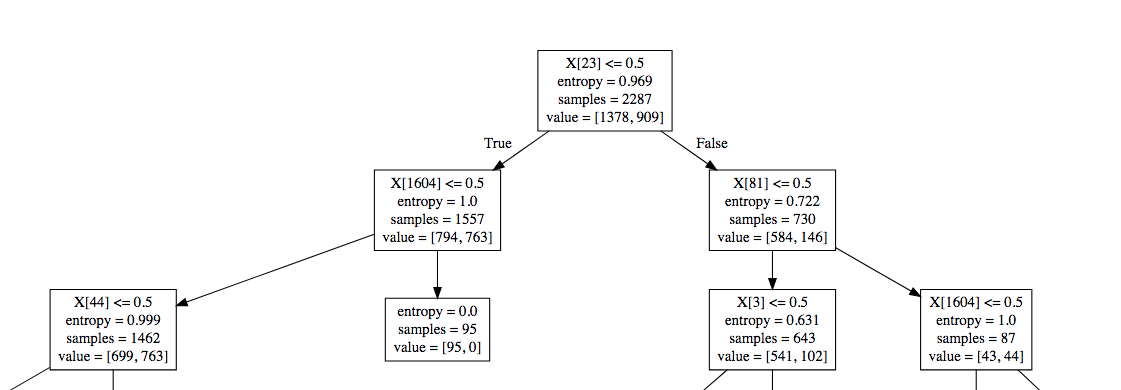
\includegraphics[width=4in]{resources/part7b}
         \caption{The top few layers of the decision tree (depth = 20).}
      \end{figure}

   It is interesting to look at the words being split on in these layers; $X$ was a list of all words
   that appeared in either the fake or real datasets. These words are `donald' (23), `trumps' (1604; note the
   double appearance), `the' (81), `hillary' (44), and `trump' (3). The exact same process of training was run
   ignoring stop words, but results were slightly worse; graphs similar to those mentioned above can be found
   in the \texttt{resources} directory (each filename indicates whether stop words were included).

   Note that as one moves down the tree, the entropy reduces, which is to be expected - the words that give
   the highest gain are split on first. A visualization of the entire tree is saves as \texttt{part7b_all.pdf}
   in the \texttt{resources} directory; the text represenations of many trees that were generated during
   training are saved in \texttt{resources/part7}.

   \subsection{Comparison of All 3 Classifiers}
   All three classifiers preform much better than random guessing...


   \section{Information Theory}




\end{document}
